\documentclass[12pt,a4paper]{article}

\usepackage{fontawesome5}
\providecommand{\faPencilAlt}{\faIcon{pencil-alt}}

\usepackage{styles/couleurs}
\usepackage{styles/mise_en_page}
\usepackage{styles/boites}
\usepackage{styles/maths}
\usepackage{styles/figures}

\usepackage{enumitem}
\usepackage{array}
\usepackage{tabularx}
\usepackage{amsmath}
\usepackage{amssymb}
\usepackage{tikz}
\usepackage{xparse}
\usepackage{pdflscape}
\usepackage{colortbl}

\usetikzlibrary{calc,arrows.meta,positioning}

\setlist[itemize]{leftmargin=1.4em,itemsep=0.15em,topsep=0.2em}
\setlist[enumerate]{leftmargin=*,itemsep=0.22em,topsep=0.25em}

\newcommand{\lignepointillee}{\noindent\dotfill\par\vspace{0.45em}}

\newcommand{\lignesreponse}[1]{%
\begin{tcolorbox}[
enhanced,colback=white,colframe=NeutreC!40,boxrule=0.5pt,arc=1.5mm,
left=3mm,right=3mm,top=2mm,bottom=1mm,before skip=2pt,after skip=2pt]
\foreach \i in {1,...,#1}{\lignepointillee}
\end{tcolorbox}}

\newcommand{\titreseq}[1]{%
\begin{center}
{\sffamily\LARGE\bfseries\color{TitreC}Séquence 7 -- Arithmétique}\\[0.2em]
{\sffamily\large\bfseries\color{SavoirC}#1}
\end{center}}

\newcommand{\grillecent}{%
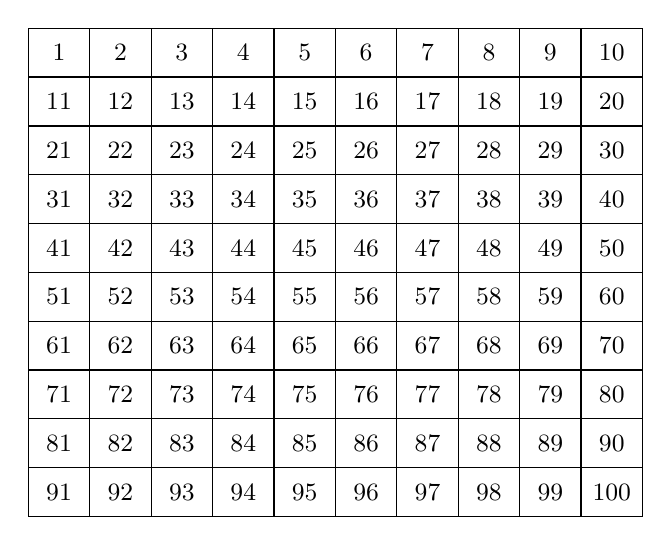
\begin{tikzpicture}[x=0.78cm,y=0.62cm]
  \foreach \n in {1,...,100}{
    \pgfmathtruncatemacro{\col}{mod(\n-1,10)}
    \pgfmathtruncatemacro{\lig}{9-floor((\n-1)/10)}
    \draw[line width=0.45pt] (\col,\lig) rectangle ++(1,1);
    \node[font=\small] at (\col+0.5,\lig+0.5) {\n};
  }
\end{tikzpicture}}

\begin{document}

\titreseq{Activité 7 -- Mission nombres}

\remarque{Cette activité de synthèse se réalise par équipes.
Chaque mission validée donne un chiffre du code final.}

\section*{Mission 1 -- Les nombres premiers}

Parmi les nombres suivants, recopie uniquement les nombres premiers :

\[
51\qquad 53\qquad 57\qquad 61\qquad
67\qquad 69\qquad 71\qquad 77.
\]

Pour chaque nombre écarté, donne un diviseur différent de \(1\)
et de lui-même.

Le premier chiffre du code est le nombre de nombres premiers trouvés.

\lignesreponse{5}

\section*{Mission 2 -- Le nombre mystérieux}

Je suis un entier compris entre \(100\) et \(400\).

\begin{itemize}
  \item Je suis pair.
  \item Je suis divisible par \(11\).
  \item \(3\) et \(5\) sont aussi mes diviseurs.
\end{itemize}

Qui suis-je ? Justifie sans tester tous les entiers.

Le deuxième chiffre du code est mon chiffre des dizaines.

\lignesreponse{5}

\section*{Mission 3 -- Décomposition}

Décompose \(396\) en produit de facteurs premiers.

Le troisième chiffre du code est le nombre total de facteurs premiers
écrits dans la décomposition, en comptant les répétitions.

\lignesreponse{5}

\section*{Mission 4 -- Fraction}

Simplifie :

\[
\frac{84}{126}.
\]

Le quatrième chiffre du code est le dénominateur de la fraction obtenue.

\lignesreponse{5}

\section*{Mission 5 -- Vrai ou faux ?}

Pour chaque affirmation, réponds par vrai ou faux et justifie.

\begin{enumerate}
  \item Tout nombre impair est premier.
  \item Le seul nombre premier pair est \(2\).
  \item Si un nombre est divisible par \(6\), alors il est divisible par \(3\).
  \item La somme de deux nombres premiers est toujours première.
  \item Un entier supérieur à \(1\) peut toujours être décomposé
        en produit de facteurs premiers.
\end{enumerate}

\lignesreponse{7}

\section*{Bilan individuel}

Rédige deux phrases :

\begin{enumerate}
  \item une méthode pour montrer qu'un nombre n'est pas premier ;
  \item une méthode pour simplifier une fraction à l'aide
        des facteurs premiers.
\end{enumerate}

\lignesreponse{4}

\end{document}
